
\chapter{Jeu de données de la base OLTP}
\section{Modèle relationnel}
\subsection{Présentation}

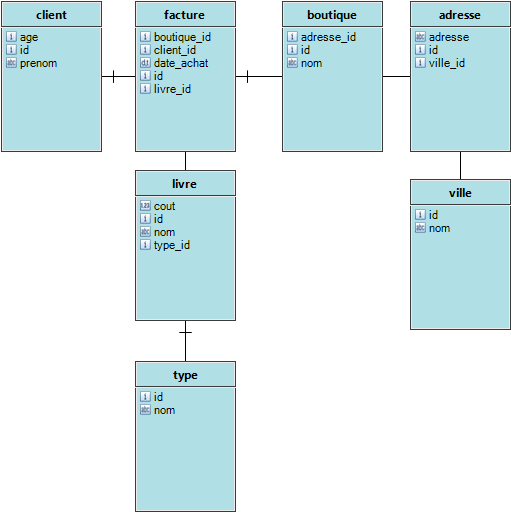
\includegraphics[clip=true, width=120mm, height=80mm]{./images/library.png}

Le modèle relationnel est un modèle normalisé. 
\begin{itemize}
\item Une facture a été établie pour un client donné dans une boutique donnée à une date donnée et en rapport avec un livre donné. 
\item Le livre appartient à un type donné (Roman, BD, etc.). 
\item La boutique a une adresse située dans une ville
\end{itemize}


Voici combien de lignes ont chaque table :
\begin{itemize}
\item adresse : 26
\item boutique : 25
\item client : 8819
\item facture : 8819
\item livre : 8
\item type : 3
\end{itemize}


En annexe \ref{generateDataR} , le code R qui a servi à générer les données dont il a été estimé que la pertinence n'avait que peu d'importance pour l'exercice.
De plus, nous possédons un fichier de type csv contenant un dictionnaire de villes avec les départements associés ainsi que les régions.
Voici en exemple les quatre premières lignes de ce fichier villes\_def.csv

\lstset{language=bash}
\lstset{frame=shadowbox}
\begin{lstlisting}
 "ville","departement","region_name"
 "Beauvais","Oise","Picardie"
 "Compiegne","Oise","Picardie"
 "Clermont","Oise","Picardie"
\end{lstlisting}

\clearpage


